\documentclass[12pt, letterpaper]{article}
\usepackage[spanish]{babel}
\usepackage[utf8]{inputenc}
\usepackage{graphicx}
\usepackage{amssymb}
\graphicspath{{./imagenes/}}
\usepackage{xcolor}

%Paquetes para símbolos y entornos matematicos. En este documento se usa para poder usar el tag \begin{align} y \begin{align*} que permiten alinear expresiones matemáticas
\usepackage{amsmath}
\usepackage{amssymb}
%paquete que permite el uso de del argumento H al momento de insertar imágenes
\usepackage{float}

%comando para especificar el título del documento 
\title{Matemáticas para las Ciencias Aplicadas I}

%comando para especificar el autor del documento
\author{Pérez Romero Natalia Abigail}

%comando para especificar la fecha del documento
\date{\today}
%--------------Fin preámbulo--------------

%------------Inicio documento-------------
\begin{document}
%comando que genera el titulo con los datos especificados en el preámbulo
\maketitle
\textbf{Tarea IX. Ejercicios del libro Cálculo. Una variable de Thomas J.R, George B.}

\textbf{Ejercicios  37, 50, 51, 56 y 59 de la sección 2.2 Cálculo de Límites}

\textbf{37.}
Suponga que $\lim_{x \to 0} f(x) = 1$ y $\lim_{x \to 0} f(x) = -5$. Señale qué reglas del teorema 1 se usa para realizar los pasos (a), (b) y (c) del cálculo siguiente.\\

\begin{figure}[ht]
\centering
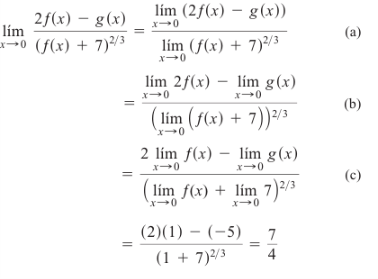
\includegraphics[width=20em]{t9uno}
\end{figure}

\textbf{a)} Regla del cociente  $\lim_{x \to c} \frac{f(x)}{g(x)} = \frac{L}{M}$ \\
\textbf{b)} En el numerador: Regla de la diferencia $\lim_{x \to c} (f(x)-g(x)) = L - M$\\
En el denominador: Regla de la potencia $\lim_{x \to c} (f(x))^{\frac{r}{s}} = L ^{\frac{r}{s}}$\\
\textbf{c)} En el numerador se aplica Regla del múltiplo constante $\lim_{x \to c} (k * f(x)) = k * L$\\
En el denominador Regla de la suma $\lim_{x \to c} (f(x)+g(x)) = L + M$\\


\textbf{50.} Si $2 - x^2 \leq g(x) \leq 2$ $cos (x)$ para toda $x$, encuentre $\lim_{x \to 0} g(x)$\\
Si  $\lim_{x \to 0} 2 - x^2 = \lim_{x \to 0} 2 - (0)^2 = 2$\\  
y  $\lim_{x \to 0} 2 \cos x = \lim_{x \to 0} 2 \cos 0 = 2$\\

El $\lim_{x \to 0} g(x) = 2$

Por el teorema del sandwich
Suponemos que $g(x) \leq f(x) \leq h(x)$ para toda $x$ en algun intervalo abierto que contenga en $c$, excepto en $x = c$. Supongamos también $\lim_{x \to c} g(x) = \lim_{x \to c} h(x) = L $. Entonces $\lim_{x \to c} f(x)= L$

\textbf{51.a.} Se puede probar que las desigualdades 

\begin{align*}
	1 - \frac{x^2}{6} < \frac{x \sen x}{2-2 \cos x} < 1
\end{align*}
son válidas para toda x cercana a cero. ¿Esto nos indica algo
acerca del
$\lim_{x \to 0} \frac{x \sen x}{2-2 \cos x}$ ?

Sí\\
Tenemos $\lim_{x \to 0} 1 - \frac{x^2}{6} = \lim_{x \to 0} 1 =1$\\ 
Debido al teorema del sandwich:\\
$\lim_{x \to 0} \frac{x \sen x}{2-2 \cos x} = 1$\\


\textbf{51.b.} Grafique en una misma gráfica las ecuaciones\\
$y = (1 - \frac{x^2}{6})$, $y = \frac{(x \sen x)}{(2 - 2 \cos x)}$ y $y = 1$ 
en una misma gráfica para $-2 \leq 2 \leq 1$. Comente el comportamiento de las gráficas cuando $x \to 0$
\begin{figure}[ht]
\centering
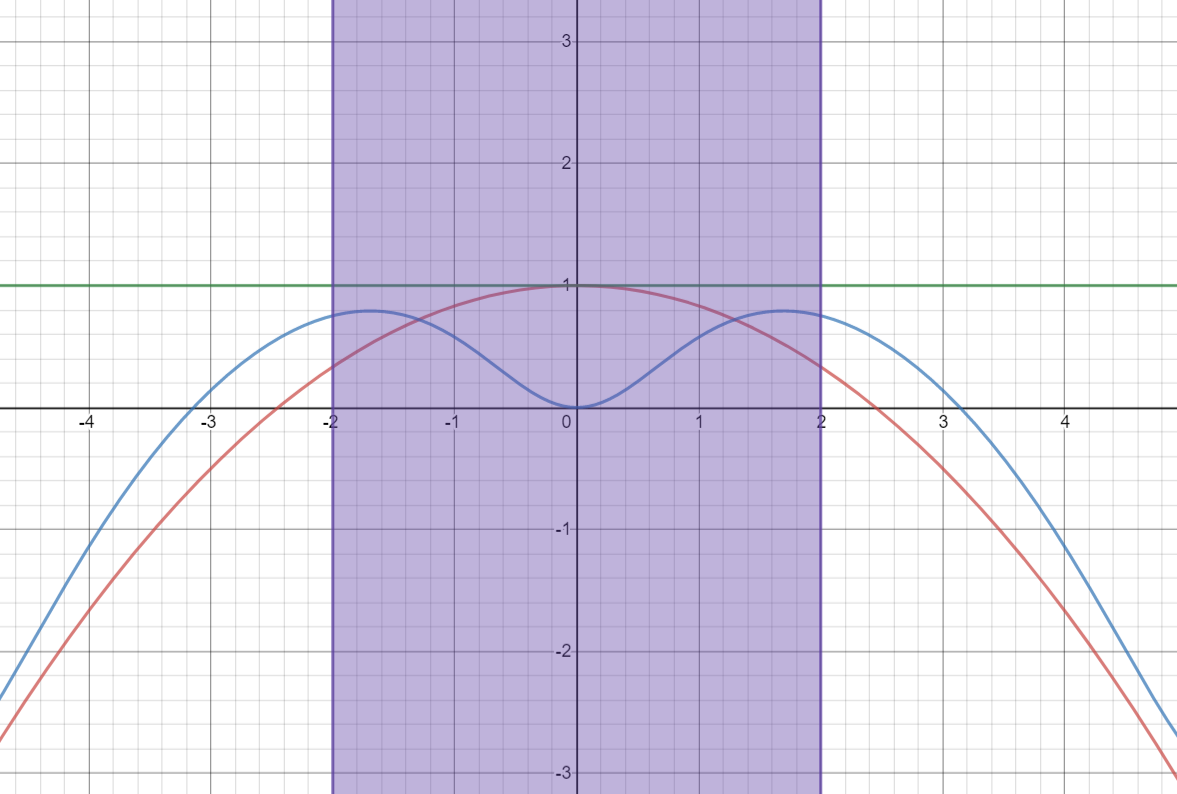
\includegraphics[width=20em]{t9dos}
\caption{\textcolor{red}{$y = (1 - \frac{x^2}{6})$}, \textcolor{blue}{$y = \frac{(x \sen x)}{(2 - 2 \cos x)}$} y  \textcolor{green}{$y = 1$ }}	
\end{figure}
Cuando $x \to 0 y = \frac{(x \sen x)}{(2 - 2 \cos x)}$ tiende a 0, $y = (1 - \frac{x^2}{6})$ y $y = 1$ cuando $x$ tiende a 0 $y$ tienden a 1

\textbf{56.} Si $\lim_{x \to -2} \frac{f(x)}{x^2} = 1$, encuentre\\

$\lim_{x \to -2} \frac{f(x)}{x^2} = \lim_{x \to -2} \frac{f(-2)}{(-2)^2} = \lim_{x \to -2} \frac{f(-2)}{4} = 1$, para que $f(-2)/4=1$, $f(-2) = 4$, entonces  $f(x)$ puede ser $-2x$

\textbf{a.} $\lim_{x \to -2} f(x) = f(-2)$ puede ser a $-4$
\textbf{b.} $\lim_{x \to -2} \frac{f(x)}{x} = \frac{f(-2)}{-2}$ puede ser $-4/-2 = 2$

\textbf{59.a} Grafique $g(x) = x \sen (1/x)$ para estimar $\lim_{x \to 0} g(x)$, acercándose al origen tanto como sea necesario.\\
\begin{figure}[ht]
\centering
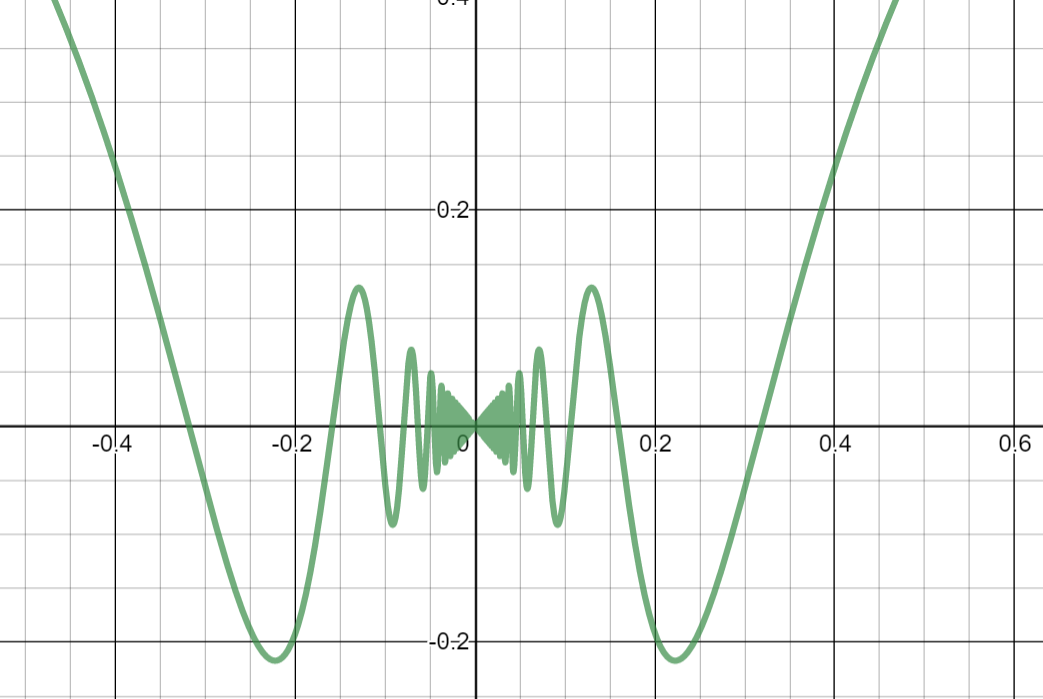
\includegraphics[width=20em]{t9tres}
\caption{\ \textcolor{green}{$g(x) = x \sen (1/x)$}}
\end{figure}
$\lim_{x \to 0} g(x) = 0$
\newpage

\textbf{59.b} Confirme mediante una prueba el resultado que obtuvo en el inciso(a)\\
Para verificar graficamente que  $\lim_{x \to 0} g(x) = 0$, analizamos la función como una composición:

\begin{figure}[ht]
\centering
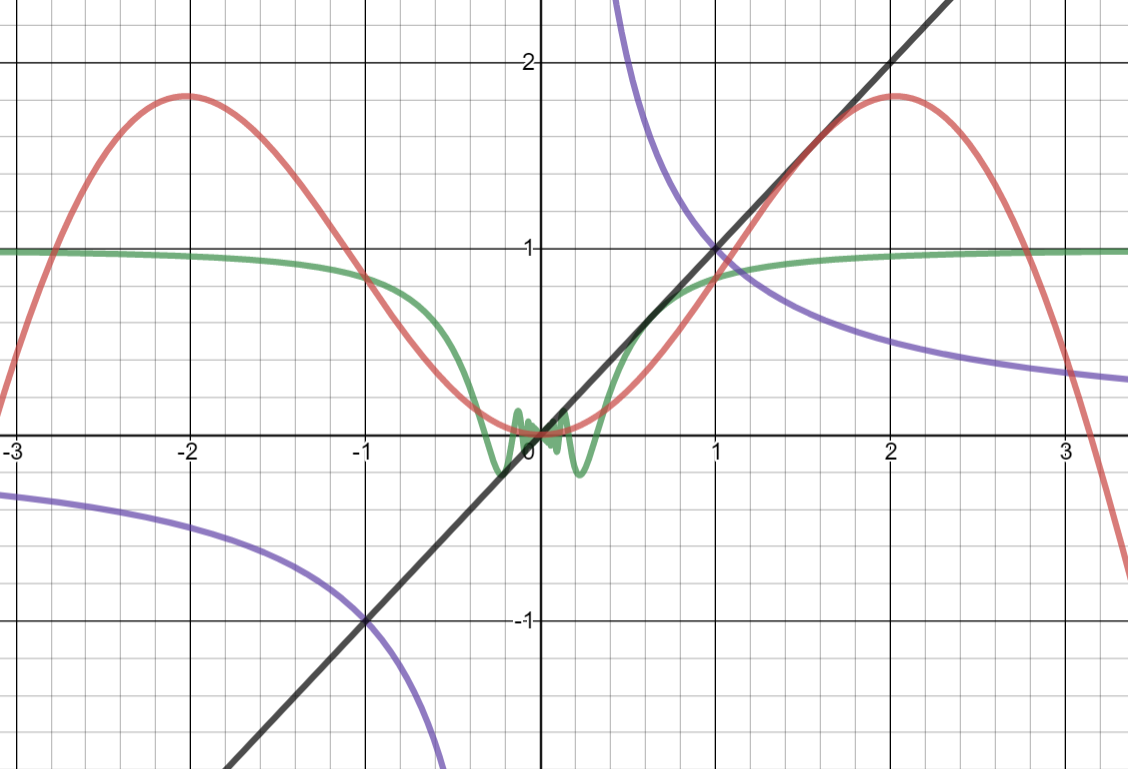
\includegraphics[width=20em]{t9cuatro}
\caption{\textcolor{violet}{$y = \frac{1}{x}$}, \textcolor{red}{$y = x\sen (x)$}, \textcolor{green}{$g(x) = x \sen (1/x)$}, $y =x$}
\end{figure}

Graficamente podemos observar que al realizar la composión de \textcolor{violet}{$y = \frac{1}{x}$}, \textcolor{red}{$y = x\sen (x)$} las x tendrán a ser muy pequeñas al acercase al 0, la función que acentúa este efecto es \textcolor{red}{$y = x\sen (x)$} debido a que es muy similar a la función identidad en la $0 \leq x \leq 1$, pero en $x > 0$ la función deja de acercarse a 0, y tiene a 1, la cual es una asíntota. Probablemente la funcíon tiende a 1 en las $x > 0$ porque $(-1,1)$ es el rango de la función seno.

Es importante notar que \textcolor{red}{$y = x\sen (x)$} también es una función compuesta: por $y = x$ y $y = \sen 1/x$

Podemos notar que \textcolor{red}{$y = x\sen (x)$} es periodica debido a a la función \textcolor{blue}{$\sen x$}, y tiene crestas que se hacen más pequeñas debido a \textcolor{violet}{$y = \frac{1}{x}$}
\begin{figure}[htb]
\centering
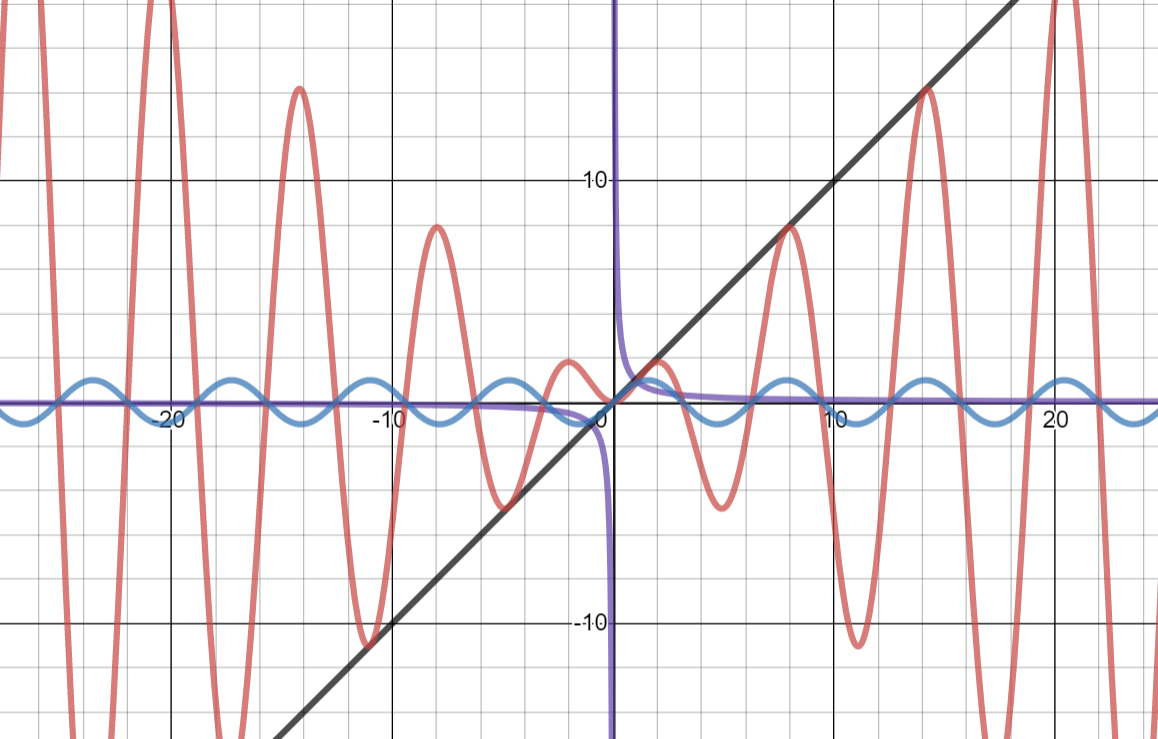
\includegraphics[width=20em]{t9cinco}
\caption{\textcolor{violet}{$y = \frac{1}{x}$}, \textcolor{red}{$y = x\sen (x)$}, $y =x$, \textcolor{blue}{$\sen x$}}
\end{figure}

\end{document}